\chapter{Конструкторская часть}

В данном разделе будут представлены требования к программе, схемы алгоритмов умножения матриц: стандартного алгоритма, алгоритма Винограда, алгоритма Штрассена и оптимизированного алгоритма Винограда.

\section{Требования к программе}
К программе предъявляются следующие требования.
\begin{itemize}
	\item Программа должна предоставлять 2 режима работы: режим умножения матриц между введёнными пользователем двумя строками и режим замера процессорного времени выполнения умножения матриц.
	\item В начале работы программы пользователю нужно ввести целое число --- это выбор пункта меню.
\end{itemize}

К первому режиму работы программы предъявляются следующие требования:
\begin{itemize}
	\item если пункт меню --- число от 1 до 4, то умножить матриц, для этого надо ввести две матрицы;
	\item программа должна вывести результирующую матрицу.
\end{itemize}

Ко второму режиму работы программы предъявляются следующие требования:
\begin{itemize}
	\item если пункт меню --- число от 5 до 7, то провести замеры времени и памяти умножения матриц каждого алгоритма;
	\item матрицы генерируются автоматически.
\end{itemize}

\section{Разработка алгоритмов}

На рисунке \ref{img:standard} приведена схема стандартного алгоритма умножения матриц. 
Схема умножения матриц по алгоритму Винограда приведена на рисунках \ref{img:winograd1}-\ref{img:winograd2},
Схема умножения матриц по алгоритму Штрассена приведена на рисунка \ref{img:strassen1}-\ref{img:strassen}, схема оптимизированной версии приведена на рисунках \ref{img:optimized_winograd1}-\ref{img:optimized_winograd2}.
\begin{figure}[H]
	\begin{center}
		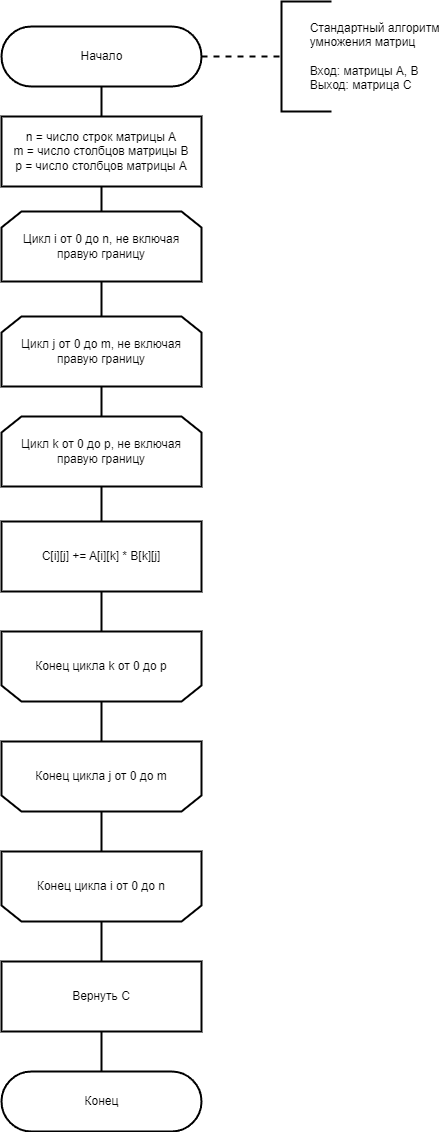
\includegraphics[scale=0.6]{img/standard.png}
	\end{center}
	\captionsetup{justification=centering}
	\caption{Стандартный алгоритм умножения матриц}
	\label{img:standard}
\end{figure}

\begin{figure}[H]
	\begin{center}
		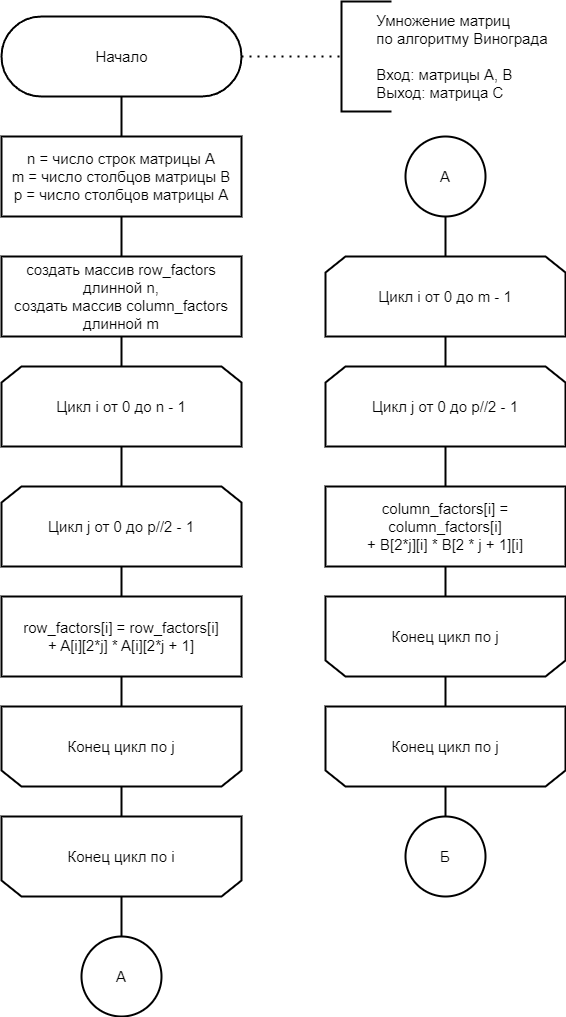
\includegraphics[scale=0.6]{img/winograd1.png}
	\end{center}
	\captionsetup{justification=centering}
	\caption{Умножение матриц по алгоритму Винограда}
	\label{img:winograd1}
\end{figure}

\begin{figure}[H]
	\begin{center}
		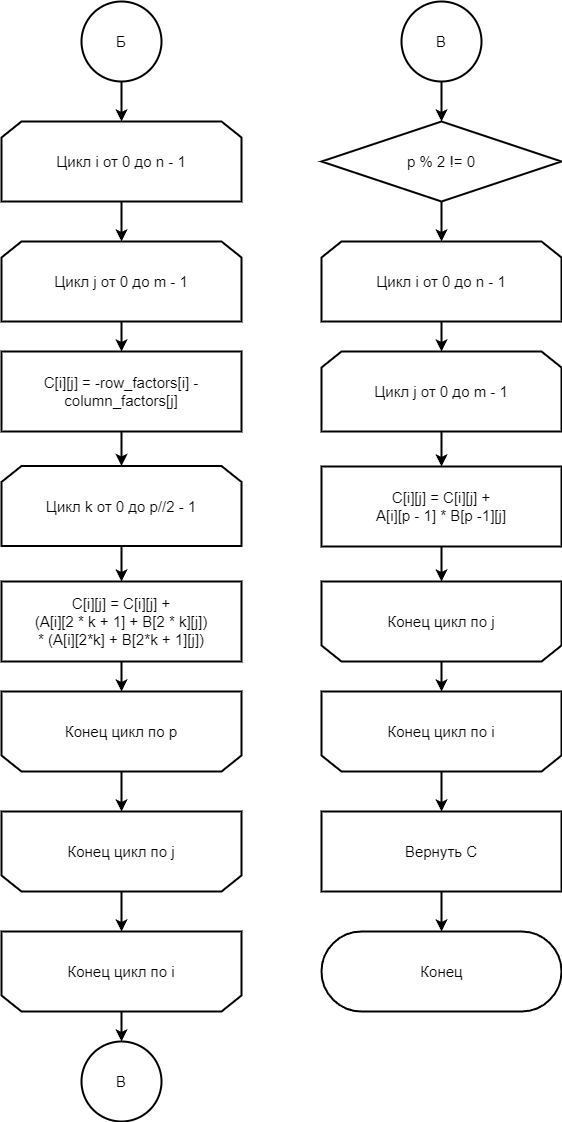
\includegraphics[scale=0.6]{img/winograd2.png}
	\end{center}
	\captionsetup{justification=centering}
	\caption{Умножение матриц по алгоритму Винограда (продолжение)}
	\label{img:winograd2}
\end{figure}

\begin{figure}[H]
	\begin{center}
		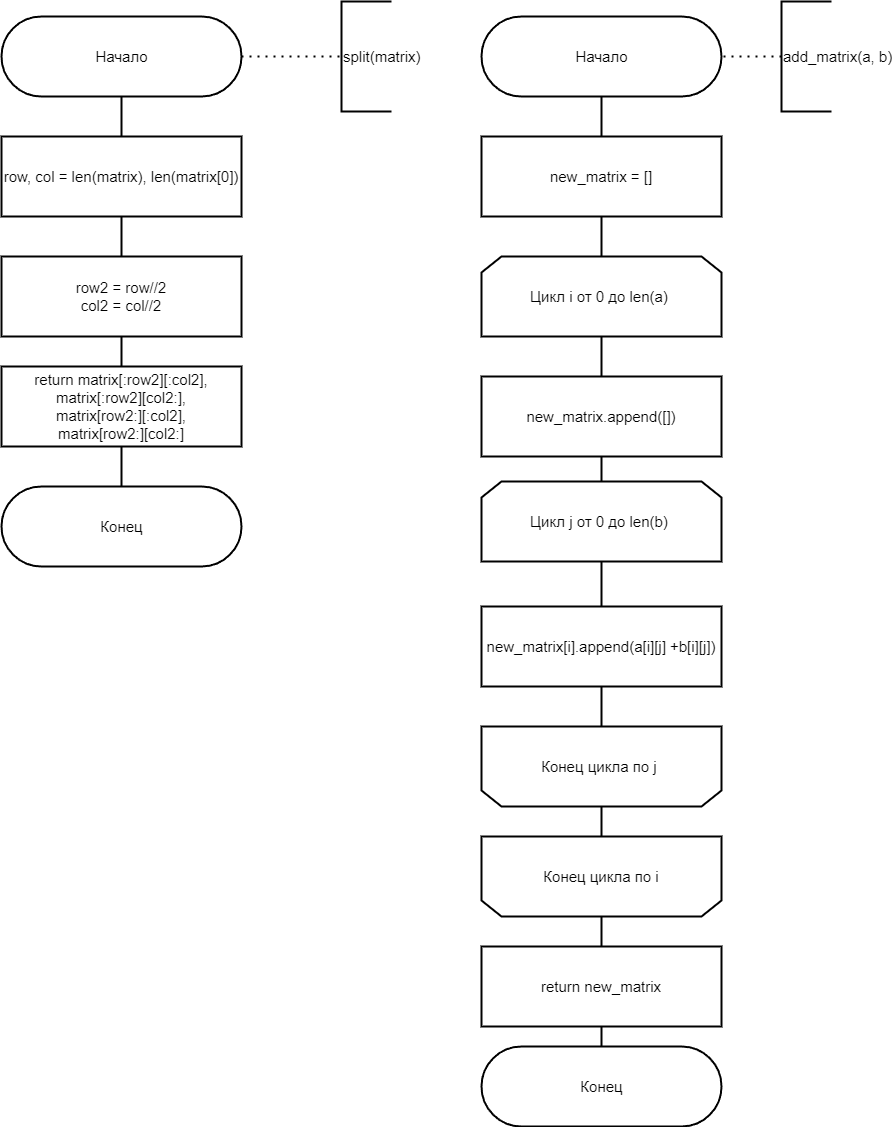
\includegraphics[scale=0.5]{img/strassen1.png}
	\end{center}
	\captionsetup{justification=centering}
	\caption{Функции разделения матрицы и сложение матриц}
	\label{img:strassen1}
\end{figure}

\begin{figure}[H]
	\begin{center}
		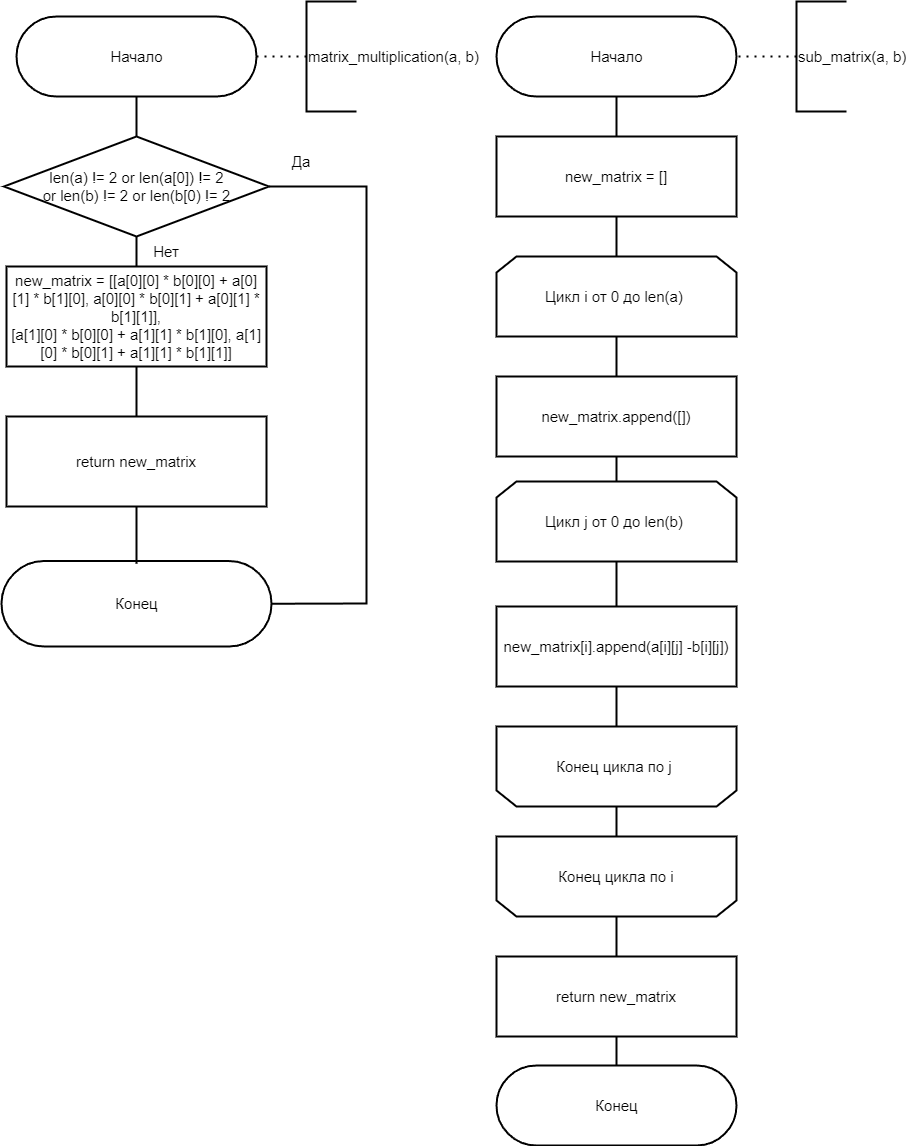
\includegraphics[scale=0.5]{img/strassen2.png}
	\end{center}
	\captionsetup{justification=centering}
	\caption{Функция умножение матрица размер 2x2 и функция вычитание матриц}
	\label{img:strassen2}
\end{figure}

\begin{figure}[H]
	\begin{center}
		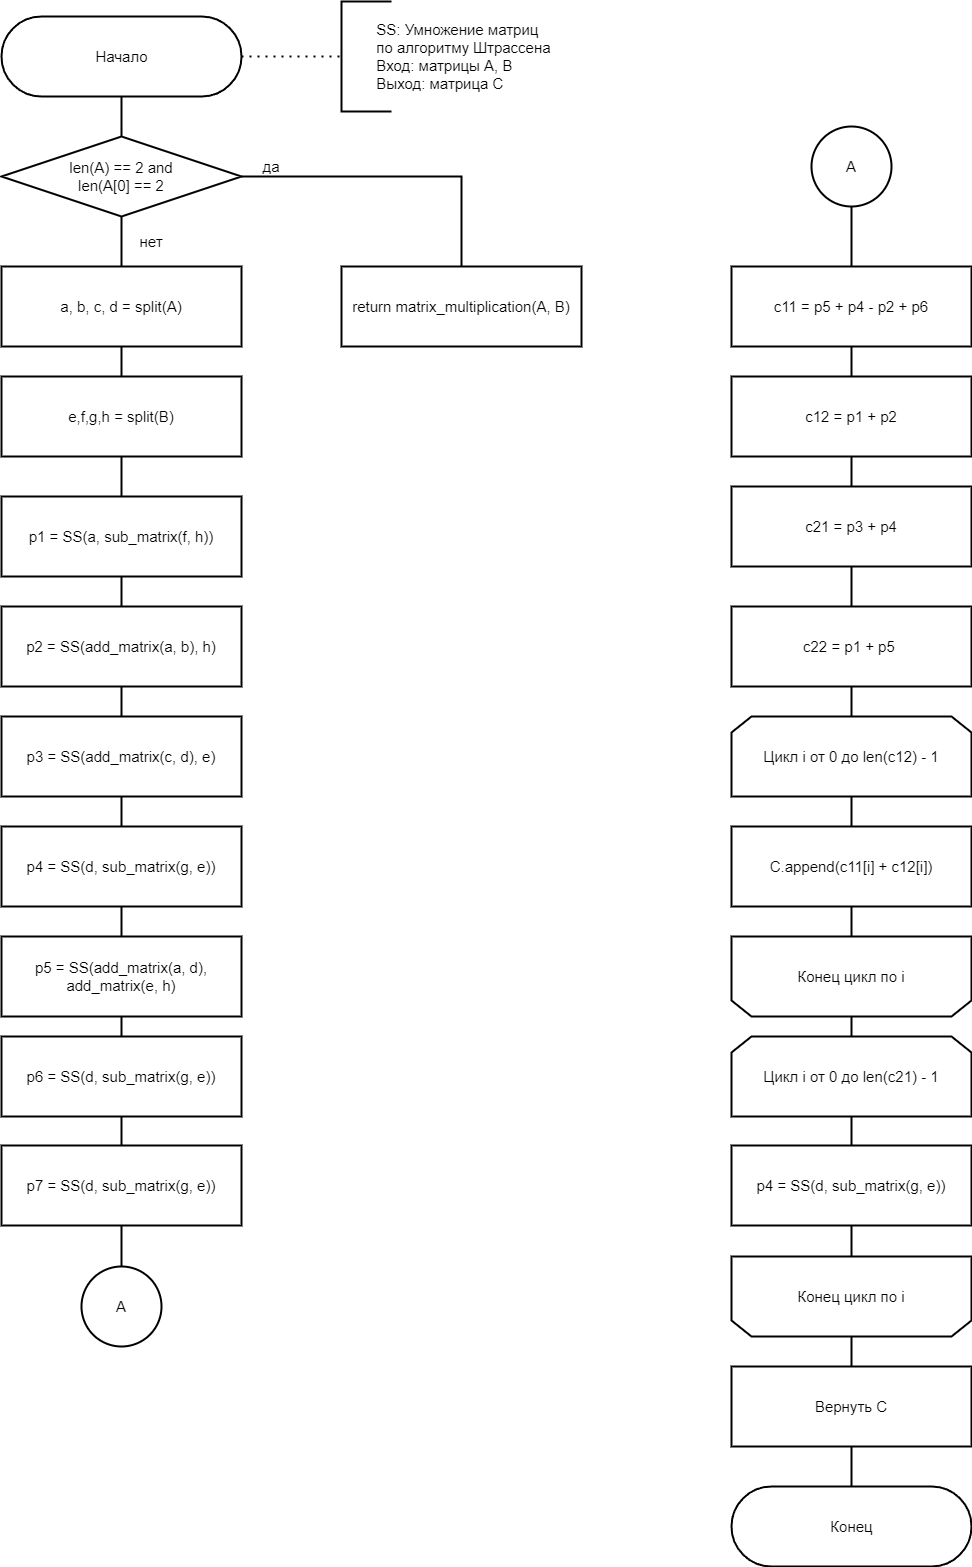
\includegraphics[scale=0.4]{img/strassen.png}
	\end{center}
	\captionsetup{justification=centering}
	\caption{Вычисление результата умножения матриц по алгоритму Штрассена}
	\label{img:strassen}
\end{figure}

\begin{figure}[H]
	\begin{center}
		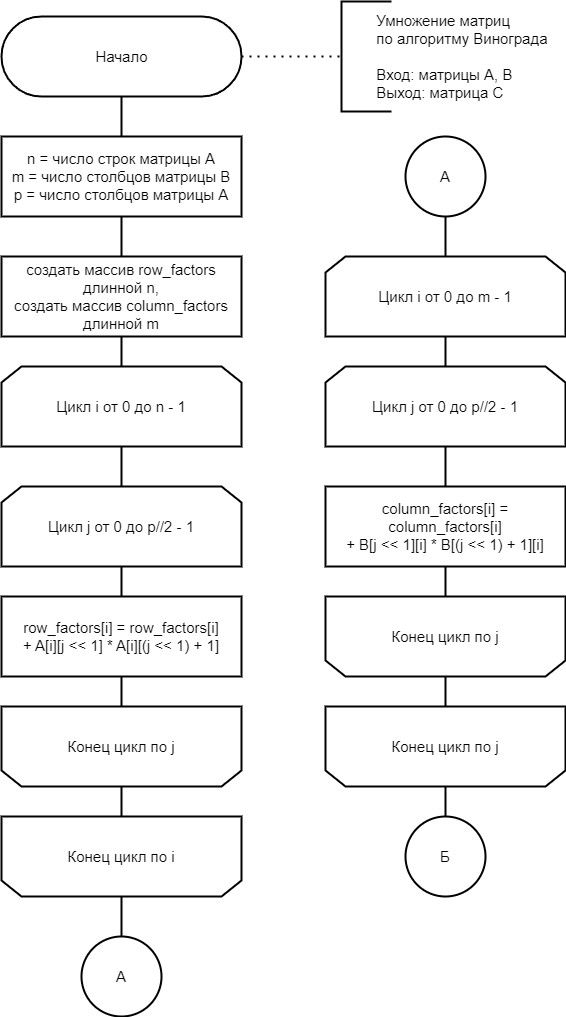
\includegraphics[scale=0.6]{img/optimized_winograd1.png}
	\end{center}
	\captionsetup{justification=centering}
	\caption{Умножение матриц по оптимизированному алгоритму Винограда}
	\label{img:optimized_winograd1}
\end{figure}

\begin{figure}[H]
	\begin{center}
		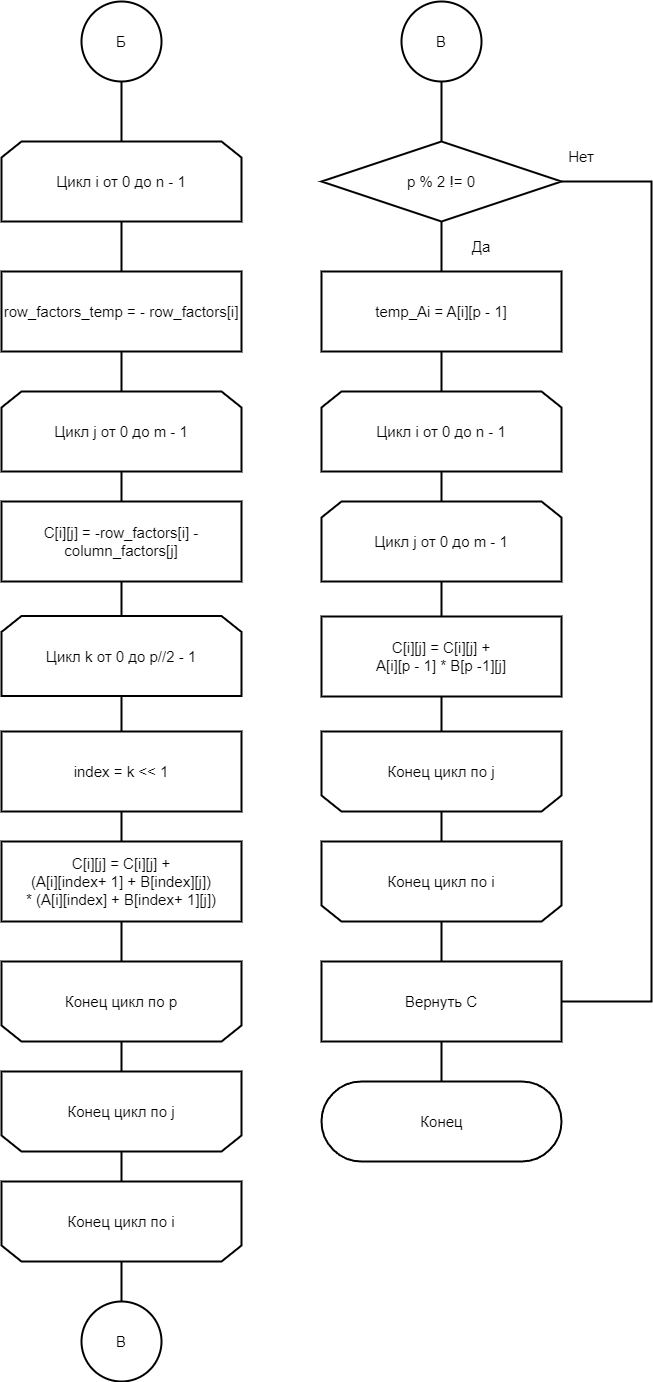
\includegraphics[scale=0.5]{img/optimized_winograd2.png}
	\end{center}
	\captionsetup{justification=centering}
	\caption{Умножение матриц по оптимизированному алгоритму Винограда (продолжение)}
	\label{img:optimized_winograd2}
\end{figure}


\section{Модель вычислений для оценки трудоемкости алгоритмов}

Для определения трудоемкости алгоритмов необходимо ввести модель вычислений \cite{model}:

\begin{enumerate}
	\item операции из списка (\ref{for:operation1}) имеют трудоемкость равную 2;
	\begin{equation}
		\label{for:operation1}
		*, /, \%, *=, /=, \%=
	\end{equation}
	\item операции из списка (\ref{for:operations2}) имеют трудоемкость равную 1;
	\begin{equation}
		\label{for:operations2}
		+, -, +=, -=, =, ==, !=, <, >, <=, >=, [], ++, {-}-
	\end{equation}
	\item трудоемкость оператора выбора \code{if условие then A else B} рассчитывается, как (\ref{for:if});
	\begin{equation}
		\label{for:if}
		f_{if} = f_{\text{условия}} +
		\begin{cases}
			f_A, & \text{если условие выполняется,}\\
			f_B, & \text{иначе.}
		\end{cases}
	\end{equation}
	\item трудоемкость цикла рассчитывается, как (\ref{for:cycle});
	\begin{equation}
		\label{for:cycle}
		f_{for} = f_{\text{инициализации}} + f_{\text{сравнения}} + N(f_{\text{тела}} + f_{\text{инкремент}} + f_{\text{сравнения}})
	\end{equation}
	\item трудоемкость вызова функции равна 0.
\end{enumerate}

\section{Трудоемкость алгоритмов}

Проведем сравнительный анализ реализованных алгоритмов по трудоемкости для умножения матрицы A[N][P] и матрицы B[P][M].

\subsection{Стандартный алгоритм умножения матриц}

Трудоемкость данного алгоритма будет складываться из:

\begin{itemize}
	\item трудоемкости цикла по $k \in [0..P-1]$, равной $2 + P(2 + 1 + 8 + 1 + 2) = 2 + 14P$;
	\item трудоекмости цикла по $j \in [0..M-1]$, равной $2 + M(2 + f_{body}) = 2 + M(4 + 14P) = 2 + 4M + 14PM$;
	\item трудоемкости цикла по $i \in [0..N-1]$, равной $2 + N(2 + f_{body}) = 2 + N(2 + 2 + 4M + 14MP) = 2 + 4N + 4NM + 14NMP$.
\end{itemize}

Таким образом, трудоемкость стандартного алгоритма умножения равна $f_{standard} = 2 + 4N + 4NM + 14NMP \approx 14NMP$.

\subsection{Алгоритм умножения матриц по Винограду}

Трудоемкость данного алгоритма будет складываться из:

\begin{itemize}
	\item трудоемкости создания и заполнения нулями векторов row\_factors и column\_factors, равной $N + M$;
	\item трудоемкости предварительных вычислений для строк, равной $2 + N(4 + 2 + P/2(3 + 12)) = 2 + 6N + 7.5NP$;
	\item трудоемкости предварительных вычислений для столбцов, равной $2 + M(4 + 2 + P/2(3 + 12)) = 2 + 6M + 7.5MP$;
	\item трудоемкости цикла по $k \in [0..P/2-1]$, равной $4 + P/2 \cdot 30 = 4 + 15P$;
	\item трудоекмости цикла по $j \in [0..M-1]$, равной $2 + M(2 + 7 + f_{body}) = 2 + M(2 + 7 + 4 + 15P) = 2 + 15M + 15PM$;
	\item трудоемкости цикла по $i \in [0..N-1]$, равной $2 + N(2 + f_{body}) = 2 + N(2 + 2 + 15M + 14MP) = 2 + 4N + 15NM + 15NMP$;
	\item трудоемкости условия, равной $2$;
	\item трудоемкости двойного цикла добавления в случае нечетного размера матрицы, равной $2 + N(2 + 2 + M(2 + 14)) = 2 + 4N + 16NM$.
\end{itemize}

Таким образом, трудоемкость алгоритма умножения по Винограду в худшем случае (нечетный размер матрицы) равна $f_{worst} = N + M + 2(2 + 6N + 7.5M) + 2 + 4N + 15NM + 15NMP + 2 + 2 + 4N + 16NM = 10 + 21N + 15M + 21NM + 15NMP \approx 15NMP$.

Трудоемкость алгоритма умножения по Винограду в лучшем случае (четный размер матрицы) равна $f_{best} = N + M + 2(2 + 6N + 7.5M) + 2 + 4N + 15NM + 15NMP = 6 + 17N + 16M + 15NM + 15NMP \approx 15NMP$.

\subsection{Оптимизированный алгоритм умножения матриц по Винограду}

Трудоемкость данного алгоритма будет складываться из:

\begin{itemize}
	\item трудоемкости создания и заполнения нулями векторов row\_factors и column\_factors, равной $N + M$;
	\item трудоемкости предварительных вычислений для строк, равной $2 + N(4 + 2 + P/2(2 + 11)) = 2 + 6N + 6.5NP$;
	\item трудоемкости предварительных вычислений для столбцов, равной $2 + M(4 + 2 + P/2(2 + 11)) = 2 + 6M + 6.5MP$;
	\item трудоемкости цикла по $k \in [0..P/2-1]$, равной $4 + P/2(20) = 4 + 10P$;
	\item трудоекмости цикла по $j \in [0..M-1]$, равной $2 + M(2 + 4 + f_{body})$;
	\item трудоемкости цикла по $i \in [0..N-1]$, равной $2 + N(4 + f_{body})$;
	\item трудоемкости условия, равной $2$;
	\item трудоемкости двойного цикла добавления в случае нечетного размера матрицы, равной $2 + N(6 + 2 + M(2 + 8)) = 2 + 8N + 10NM$.
\end{itemize}

Таким образом, трудоемкость оптимизированного алгоритма умножения по Винограду в худшем случае (нечетный размер матрицы) равна $f_{worst} = N + M + 2(1 + 4N + 6.5M) + 2 + N(4 + 2 + M(6 + 10P + 4)) = 4 + 13N + 13M + 20MN + 10MNP \approx 9.5NMP$.

Трудоемкость оптимизированного алгоритма умножения по Винограду в лучшем случае (четный размер матрицы) равна $f_{best} = N + M + 2(1 + 4N + 6.5M) + 2 + N(4 + 2 + M(6 + 10P + 4)) + 2 + 2 + 8N + 10MN = 8 + 21N + 13M + 30MN + 10MNP \approx 9.5NMP$.

\section{Вывод}

Были представлены требования к программе, схемы алгоритмов умножения матриц.
